\documentclass[modern,letterpaper]{aastex61}

% to-do list
% ----------
% - add items here
% style notes
% -----------
% - This file generates by Makefile; don't be typing ``pdflatex'' or some bullshit.
% - Line break between sentences to make the git diffs readable.
% - Use \, as a multiply operator.
% - Reserve () for function arguments; use [] or {} for outer shit.
% - Use \sectionname not Section, \figname not Figure, \documentname not Article or Paper or paper.

% packages
\definecolor{cbblue}{HTML}{3182bd}
\usepackage{microtype}  % ALWAYS!
\usepackage{amsmath,amssymb}
\usepackage{tikz}
\usepackage{aas_macros}
\hypersetup{backref,breaklinks,colorlinks,urlcolor=cbblue,linkcolor=cbblue,citecolor=black}
\graphicspath{{.}{figures/}{../notebooks/plots/}}

% define macros for text
\newcommand{\project}[1]{\textsl{#1}}
\newcommand{\acronym}[1]{{\small{#1}}}
\newcommand{\hipparcos}{Hipparcos}
\newcommand{\gaia}{\project{Gaia}}
\newcommand{\rave}{\project{\acronym{RAVE}}}
\newcommand{\apogee}{\project{\acronym{APOGEE}}}
\newcommand{\tmass}{\project{\acronym{2MASS}}}
\newcommand{\allwise}{\project{\acronym{allWISE}}}
\newcommand{\panstarrs}{\project{\acronym{PanSTARRS}}}
\newcommand{\galex}{\project{\acronym{GALEX}}}
\newcommand{\rosat}{\project{\acronym{ROSAT}}}
\newcommand{\documentname}{Article}
\newcommand{\sectionname}{Section}
\newcommand{\figname}{Figure}
\newcommand{\eqname}{Equation}
\newcommand{\dr}{\acronym{DR1}}
\newcommand{\tgas}{\acronym{TGAS}}
\newcommand{\etal}{\textit{et al}.}

\newcommand{\objname}{moving group}
\newcommand{\groupTen}{Group 10}
\newcommand{\groupSixteen}{Group 16}

% define macros for math
\newcommand{\given}{\,|\,}
\newcommand{\normal}{{\mathcal{N}}}
\newcommand{\uniform}{{\mathcal{U}}}
\newcommand{\dd}{\mathrm{d}}
\newcommand{\transp}[1]{{#1}^{\!\mathsf{T}}}
\newcommand{\inv}[1]{{#1}^{-1}}
\newcommand{\bs}[1]{\boldsymbol{#1}}
\newcommand{\vperp}{\bs{v}^\perp}
\newcommand{\propm}{\bs{\mu}}
\newcommand{\mat}[1]{\mathbf{#1}}
\renewcommand{\vec}[1]{\bs{#1}}
\newcommand{\kms}{\ensuremath{\rm km~s^{-1}}}
\newcommand{\msun}{{\rm M}_\odot}
\newcommand{\data}{\mathrm{data}}
\newcommand{\snr}{[S/N]_\varpi}
\newcommand{\eye}{\mathbb{I}}
\newcommand{\absdvtan}{\ensuremath{|\Delta\vec v_\mathrm{t}|}}
\newcommand{\estimates}{\ensuremath{\{\hat{\varpi_i},\hat{\mu_{\alpha,i}},\hat{\mu_{\delta,i}},\hat{v_{r,i}}\}}}

\newcommand{\ra}{\text{R.A.}}
\newcommand{\dec}{\text{Decl.}}
\newcommand{\pmra}{\ensuremath{\mu_\alpha^*}}
\newcommand{\pmdec}{\ensuremath{\mu_\delta}}
\newcommand{\masyr}{\ensuremath{\mathrm{mas}\,\mathrm{yr}^{-1}}}

\definecolor{crimson}{rgb}{0.79, 0.0, 0.09}
\newcommand{\todo}[1]{{\color{crimson}#1}}

\newcommand{\groupDistanceEstimate}{\ensuremath{100~\mathrm{pc}}}
\newcommand{\groupAgeEstimate}{\ensuremath{500~\mathrm{Myr}}}
\newcommand{\totalNumberOfCandidates}{\ensuremath{29}}
\newcommand{\meanVelocityOpt}{\ensuremath{(u_x,\,u_y,\,u_z) = (-3.9,\,7.0,\,-3.8)~\kms}}
\newcommand{\sigVelocityOpt}{\ensuremath{0.42~\kms}}
\newcommand{\nstarsInRegion}{3413}
\newcommand{\bprp}{\ensuremath{\mathrm{BP}-\mathrm{RP}}}

\begin{document}\sloppy\sloppypar\raggedbottom\frenchspacing % trust me

\title{
  Rediscovery of a nearby young, coeval moving group
}

\author[0000-0001-7790-5308]{Semyeong Oh \etal}
\affiliation{Department of Astrophysical Sciences,
             Princeton University, Princeton, NJ 08544, USA}

\correspondingauthor{Semyeong Oh}
\email{semyeong@astro.princeton.edu}

\begin{abstract}

  We confirm and characterize a recently discovered, nearby ($d \approx \groupDistanceEstimate$), young (age$\approx 250$~Myr) moving group using astrometric and photometric data from \gaia\ DR 2 combined with spectroscopic data compiled from the literature.
  This group, which notably includes 81 Uma and 84 Uma, spans a large area
  on sky, $(\Delta\mathrm{R.A.},\,\Delta\mathrm{Decl.})\approx(39,\,18)$~deg,
  thus allowing for a well-constrained astrometric radial velocity that agrees with spectroscopic radial velocities for a subset of members.
  The morphology of the group is unlike that of Galactic open clusters: while relatively compact in Galactic $Z$, the group displays a $XX$~pc gap in the spatial distribution in Galactic $(X, Y)$ coordinates that may be an indication of ongoing disruption or dissolution.
  \todo{list some conclusions!}

\end{abstract}

\section{Introduction} % (fold)
\label{sec:introduction}

Comoving, coeval stars in the Solar neighborhood are valuable astrophysical
laboratories for studying stellar properties, stellar evolution, and galactic
dynamics \citep[e.g.,][]{2018arXiv180409378G,2018MNRAS.tmp.1228M}.
Multiple stars form in each molecular cloud, often in kinematically coherent
groups.
Galactic dynamics determines how and when these groups eventually dissolve into the field population.
Thus, a detailed census of these objects traces both recent star formation
history in the local volume as well as the dynamics of their disruption.
Individual star clusters or coeval moving groups are also interesting dynamical
entities themselves as their dynamical evolution is intimately tied to their
internal structure and external perturbation from the Galactic tides or giant
molecular clouds.
Finally, within $\approx 100$~pc, members of young stellar groups represent the
best samples to study dusty debris disk, exopalnets and brown dwarfs through
direct imaging.

The second data release from the \gaia mission \citep[][DR 2]{2018arXiv180409365G} marks a new era for charting the kinematic substructure and stellar populations in the solar neighborhood.
\gaia DR 2 provides parallaxes, proper motions, and precise two-band photometry of stars brighter than $G\lesssim 20.7$ as well as radial velocities for stars brighter than $G\lesssim12.5$.
\citet{2017AJ....153..257O} presents a search for comoving pairs using the
Tycho-Gaia Astrometric Solution (\tgas), a subset of \gaia\ DR~1 which provides
astrometric measurements for 2~million sources in Tycho-2 catalog ($G<12$~mag).
This comoving pairs search both recovered many of the large known nearby
comoving stellar groups, ranging from loose associations to open clusters and
identified several previously unidentified new large and small groups
\citep[see also][]{2018arXiv180409058F}.
In this paper, we focus on one of the most interesting of the coeval moving
groups discovered in \citet{2017AJ....153..257O} and use the newly released \gaia\
DR 2 to present an extended analysis of the properties.
Group 10 is the largest nearby ($\approx 100$~pc) group with little prior
discussion in the literature.
% Not sure it's fitting to separate section ...
We summarize previous analyses of the stars in Group 10 in \sectionname~\ref{sec:history},
present the data and candidate member selection in \sectionname~\ref{sec:data},
discuss the ages, kinematic modelling and morphology of the group in \sectionname~\ref{sec:analysis},
and summarize in \sectionname~\ref{sec:discussion}.

\section{Previous identifications}
\label{sec:history}

Moving group identifications are often scattered throughout the literature. We
reviewed the bibliography associated with all \tgas\ sources in
\groupTen\ from our previous selection \citep{2017AJ....153..257O} using the
Simbad database, and note previous identifications of this group.

\citet{1977ATsir.969....7L} had identified three of the A-type stars in \groupTen,
HIP 66198 (81 Uma), HIP 67231 (84 Uma), and HIP 67005, as part of
a possible open cluster composed of 7 A-type stars
(HIP 66198,
HIP 67231,
HIP 67005,
HIP 67848,
HIP 66738,
TYC 3851-606-1,
TYC 3469-497-1)
dubbed Latyshev 2 by \citet{2003stcl.book.....A}.
In a recent review, \citet{2016IAUS..314...21M} doubts the physical reality of
this putative cluster based on the lack of a convergent point and deviances in
the kinematics.
However, we will show that \emph{some} of these stars are clearly part of a distinct
kinematic structure.


\section{Data \& Sample}
\label{sec:data}

% How much of the spread in velocities is physical and how much is due to
% uncertainties in the GAIA measurements


\begin{figure}
  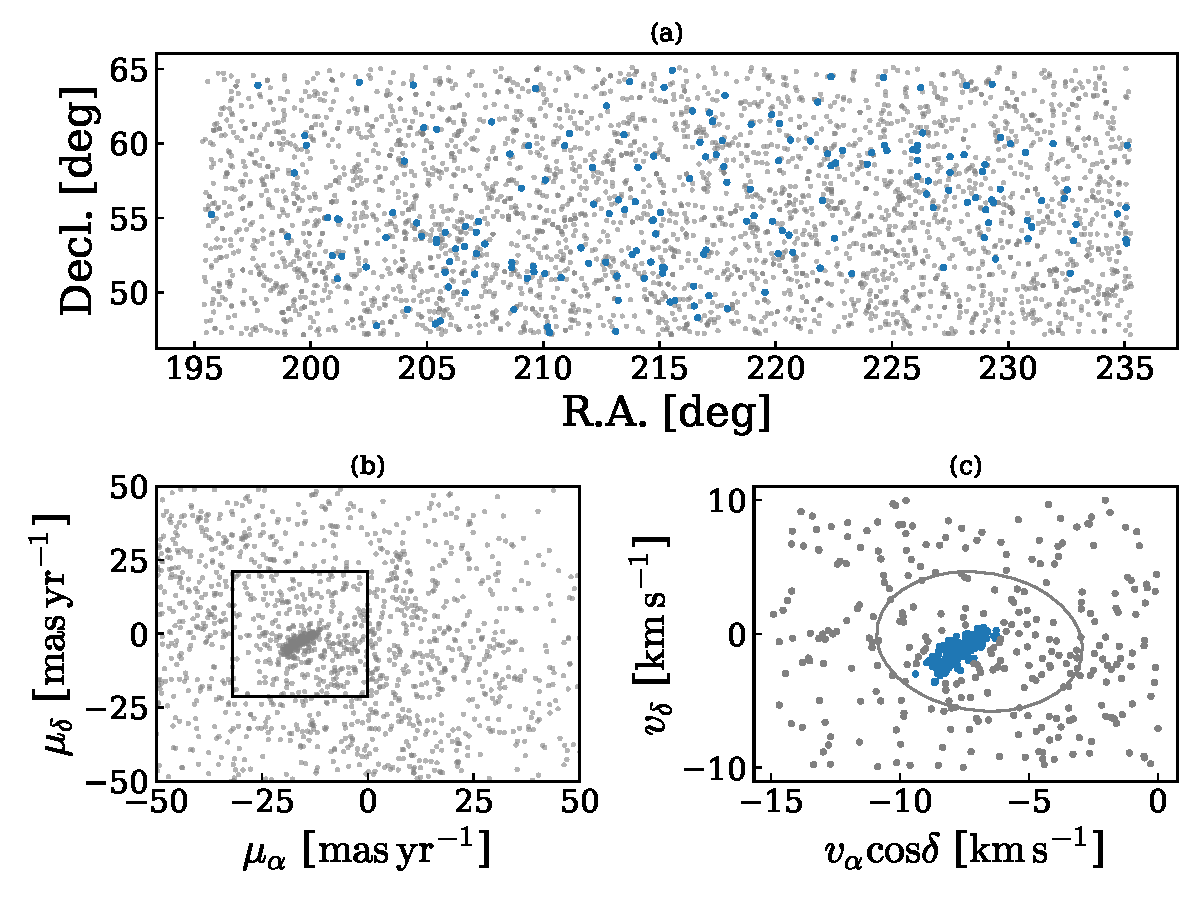
\includegraphics[width=0.95\linewidth]{g10_sky_pm.pdf}
  \caption{Distribution of stars in the neighborhood of \groupTen\
    on sky (a), in proper-motion space (b) and in tangential-velocity space (c).
    These are \nstarsInRegion\ \gaia\ sources within
    $(20,\,9)$ degrees from the mean position
    $(\mathrm{R.A.},\,\mathrm{Decl.}) = (215.32,\,56.133)$ and
    20~pc around the median parallax of $9.94$.
    We select candidate members (blue circles) by fitting two-component Gaussian
    mixture model in tangential-velocity space
    The panel (c) is a zoom-in of the box indicated in panel (b).
    See \sectionname~\ref{sec:data} for details.
    }
  \label{fig:distributions}
\end{figure}

We search for candidate members of \groupTen\ in \gaia\ DR 2
based on the angular and parallactic spread of this group from the previous
discovery using \tgas.
We go out to 20 degrees and 9 degrees from the mean position
$(\alpha,\,\delta) = (215.32,\,56.133)$
in \ra\ and \dec\ direction respectively,
and a nominal 20~pc in distance around the median parallax of $9.94$.
The exact query is
\begin{verbatim}
  select *
  from gaiadr2.gaia_source
  where
      ra between 195.320 and 235.320
      and dec between 47.134 and 65.134
      and parallax between 8.3 and 12.4
\end{verbatim}
There are \nstarsInRegion\ \gaia\ sources within these cuts.
Figure~\ref{fig:distributions} shows the distribution of these sources on sky
and in proper-motion space.
While there is no discernable concentration of sources on sky
(\figname~\ref{fig:distributions}a),
a clear overdensity is found in proper-motion space at
$(\pmra,\,\pmdec)\approx(-16.8,\,-3)~\masyr$ in agreement with the previous
identification using \tgas.
Of course, the sources in this overdensity do not have exactly the same proper
motion due to geometric projection.
The span of this overdensity in \figname~\ref{fig:distributions}b
mainly corresponds to the spread in parallaxes,
with sources with larger parallaxes having larger proper motions.

In order to select candidate members of the group,
we fit a Gaussian mixture model to the zoom-in box indicated in
\figname~\ref{fig:distributions}b in $(v_\alpha^*,\,v_\delta)$ space
with two components, one for the overdensity corresponding to the group and
one broad component for the background.
We select 194 sources with higher probability of belonging to the overdensity
component as candidate members of the group.
These sources, along with $1\sigma$ ellipse of each component of the mixture model,
are indicated in \figname~\ref{fig:distributions}c.
We expect this selection to be neither complete nor without contamination.
However, given the clear overdensity in proper-motion space within this parallax slice
of the group, we expect the contamination to be low.

Table~\ref{tab:candidates} provides all relevant \gaia\ data for the candidate members
and the combined photometry from \tmass, \allwise, and \panstarrs\
used in further analysis.
We note that 95\% of the selected candidate members have parallax
signal-to-noise ratios above 24 with median signal-to-noise ratio of 170.
From propagation of uncertainties ignoring covariances,
formal velocity uncertainties in the R.A. and Decl. directions span
$0.25$--$0.79$~\kms\ and $0.05$--$0.17$~\kms\ ($25$--$75$ percentiles).
Of 194 sources selected, there are 31 sources that have radial velocities (RVs)
measured.
The RV uncertainties are similarly small spanning $0.46$--$0.95$~\kms.
The median and standard deviation of the velocities of the 31 sources with RVs in the Galactic coordinates are $(U,\,V,\,W) = (-3.6,\,-9.1,\,-1.6)~\kms$ and $(\sigma_U,\,\sigma_V,\,\sigma_W) = (0.60,\,0.88,\,1.23)~\kms$.
In \sectionname~\ref{sec:fitting}, we derive
the isotropic velocity dispersion of the candidate members with
forward modelling.



\begin{deluxetable}{l|l|l}
  \tablecaption{Candidate members of \groupTen\ selected from \gaia\ DR 2
    \label{tab:candidates}}
  \centering
  \tablehead{
    \colhead{Column} & \colhead{Unit} & \colhead{Description}
  }
  \startdata
    source id & & \gaia\ DR 2 source id \\
    R.A. & deg & Right Ascension \\
    Decl. & deg & Declination \\
    parallax & mas & parallax \\
    pmra & \masyr\ & proper motion in R.A. direction \\
    pmdec & \masyr\ & proper motion in Decl. direction\\
    \texttt{phot\_g\_mean\_mag} & mag & \gaia\ $G$-band magnitude \\
    \texttt{phot\_bp\_mean\_mag} & mag & \gaia\ $G_\mathrm{BP}$-band magnitude \\
    \texttt{phot\_rp\_mean\_mag} & mag & \gaia\ $G_\mathrm{RP}$-band magnitude \\
    \texttt{phot\_bp\_rp\_excess\_factor} & mag & \gaia\ $G_\mathrm{RP}$-band magnitude \\
    \texttt{astrometric\_excess\_noise} &  & \\
    \texttt{tmass\_oid} & & \tmass\ source identifier\\
    $J$, $H$, $K_s$ & mag & \tmass\ photomery \\
    \texttt{allwise\_oid} & & \allwise\ source identifier\\
    W1, W2, W3, W4 & mag & \allwise\ W1, W2, W3, W4 magnitudes \\
    \texttt{obj\_id} & & \panstarrs\ source identifier\\
    $g$, $r$, $i$, $z$, $y$ & mag & \panstarrs\ photometry\\
  \enddata
\end{deluxetable}

\section{Analysis}
\label{sec:analysis}

% TODO
% I would start the analysis section with a question: is group 10 a
% single age stellar population?  This might be a better title
%
%
% Section 3.3:  Given the large area on the sky, did you have to include Oort’s
% A and B coefficients in the anlayses?
%
% Do you understand the origin of the formal (but small) difference between the two velocities?

% TODO
% Section 3.4:
%
% A thought on the orbit of the group — I think that you can argue that the
% group did not experience a close passage by a molecular cloud so that its
% median height (or more precisely its z action (Jz) ) should be close to its
% birth value.
%
% I also wonder whether the age and coldness of the group places an interesting
% constraint on any interaction with perturbs
%
% Have you fit mean velocities for the two subgroups?  How different are they?
%
% If you start with an 8 parsec diameter group and run it forward in time on
% this orbit (say following a few hundred stars), what do you find?


\subsection{Color-magnitude diagrams and isochrone ages}

\begin{figure}
  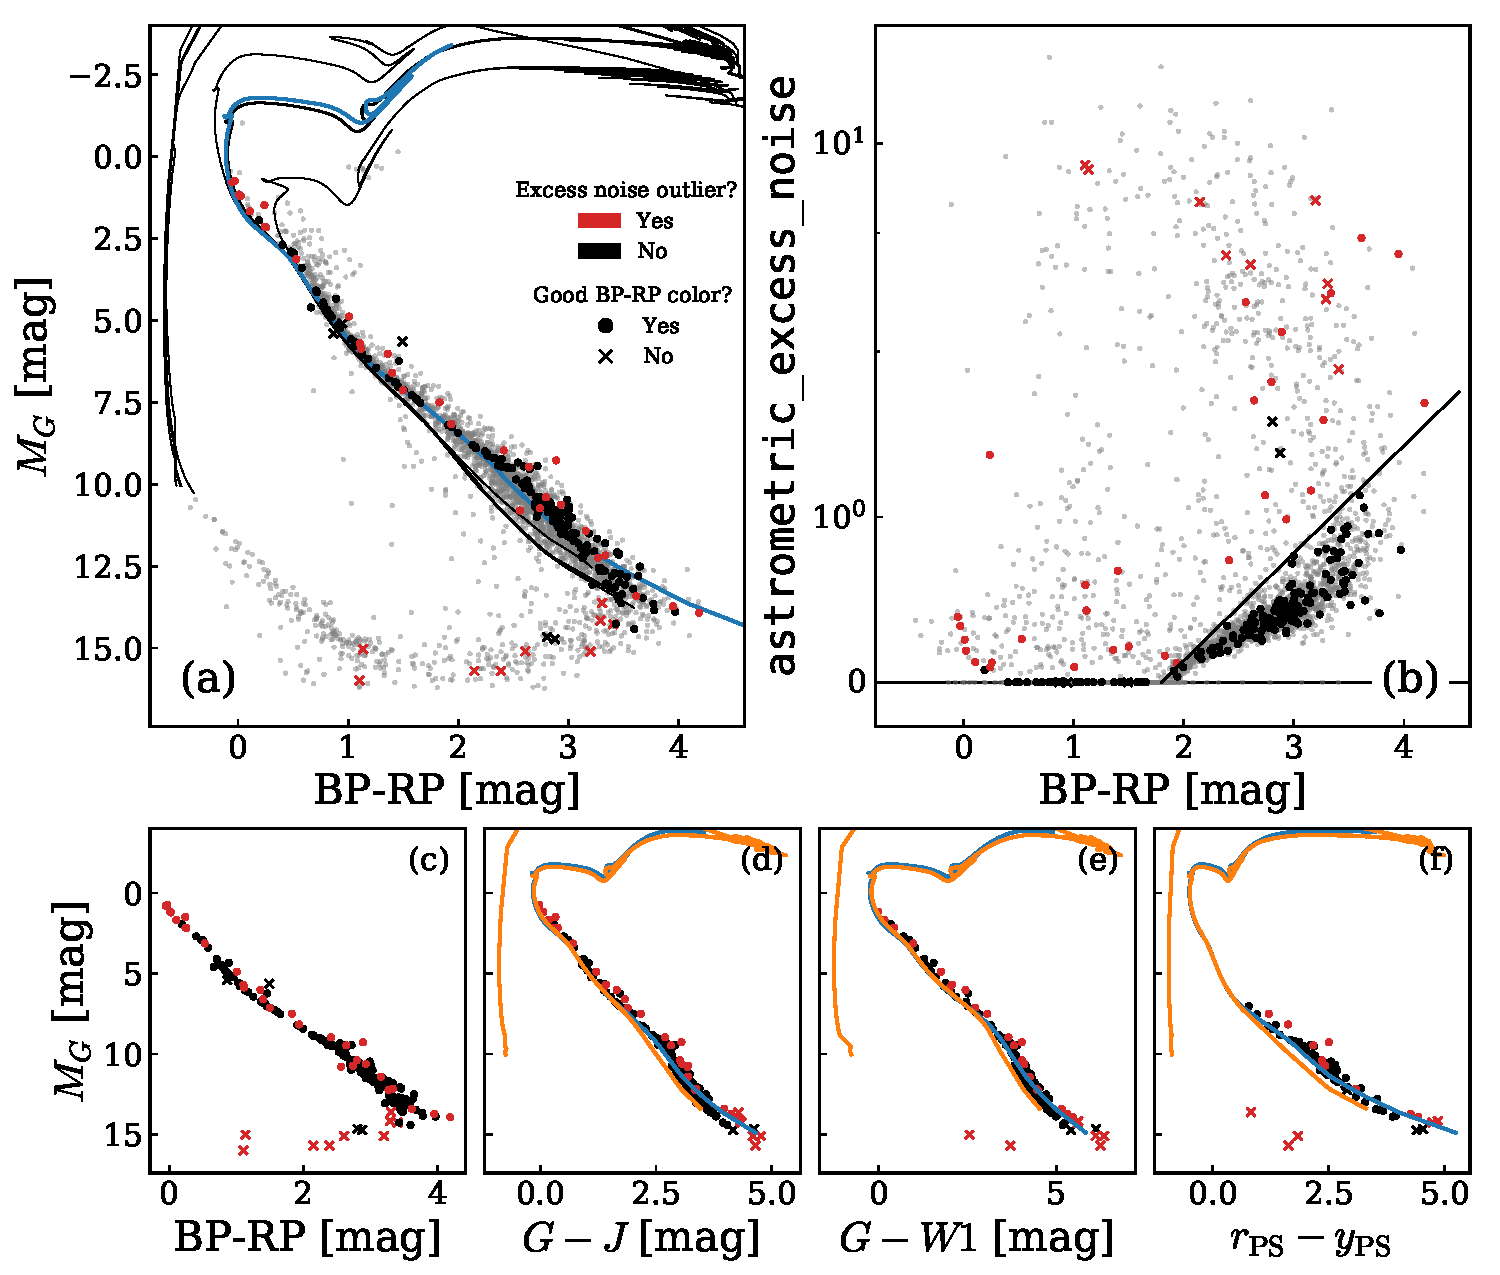
\includegraphics[width=0.95\linewidth]{bp_rp_G.pdf}
  \caption{
    Color-magnitude diagrams of candidate \groupTen\ members.
    Panel (a) and (c-e) show the color-magnitude diagram using \gaia\ (BP, RP and $G$),
    \tmass\ ($J$), \allwise\ ($W1$), and \panstarrs\ ($r_\mathrm{PS}$ and $i_\mathrm{PS}$)
    magnitudes. Panel (b) shows the astrometric excess noise from \gaia's astrometric
    solution vs. BP-RP color. The sources for which the excess noise is a significant
    outlier to the general trend (above the black line) are colored red.
    Some of the sources with bad BP, RP photometry are marked by `x'.
    Many of these seem to be low-mass stars further down the main sequence (c-e).
    Isochrones of $\log\mathrm{Age/yr}=8.4$ from MIST (black) and PARSEC (blue)
    are plotted for comparison.
    The candidate members of \groupTen\ lies on a very narrow isochrone
    compared to the density of the general field population (blue background).
  }
  \label{fig:cmd}
\end{figure}

\begin{figure}
  \centering
  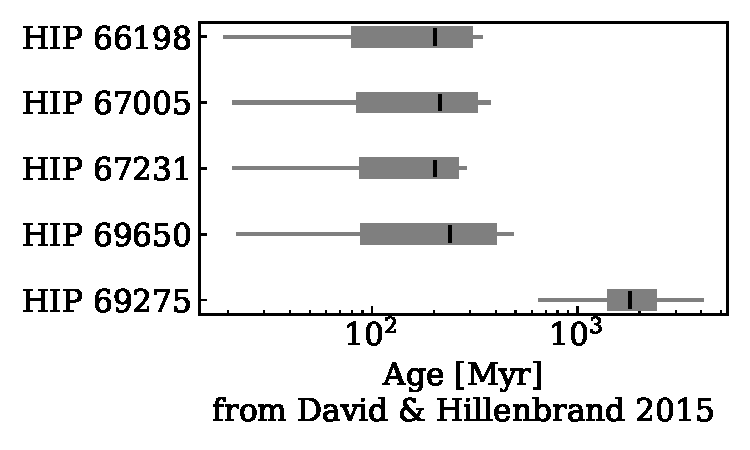
\includegraphics{age_DavidHillenbrand2015.pdf}
  \caption{Age estimates for five candidate members by \citet{2015ApJ...804..146D}.
    For each star, the black vertical line is the mode of the posterior
    distribution, and the gray band and line marks 68\% and 95\% confidence
    interval.
  }
  \label{fig:age_DavidHillenbrand2015}
\end{figure}

Figure~\ref{fig:cmd}a shows the color-magnitude diagrams of the candidate group
members using the \gaia\ photometry.
The absolute $G$ magnitude $M_G$ is calculated as $G + 5\log(\varpi) -10$ where
$\varpi$ is parallax in mas.
The group is at a high galactic latitude (median $b=55$~degrees),
and the extinction is very low.
We checked the dust maps of \citet{1998ApJ...500..525S} and
\citet{2017ApJ...846...38L}
at the location of candidate members and found the median reddening to be
$E(B-V)\lesssim 0.012$~mag although there are some variations across the region with
the maximum reddening of 0.025~mag.
We applied no correction for dust to the data or isochrone models.

The candidate members (black and red circles) resemble a clean single-age population
that lies on a very narrow main-sequence compared to the ``field'' stars within $100$~pc.
The field sample was constructed by querying all stars with parallax $\varpi>10$~mas,
parallax signal-to-noise ratio over 50 and good \bprp\ colors filtered by
\texttt{phot\_bp\_rp\_excess\_factor} accordning to cuts in \citet{2018arXiv180409378G}.

How old is \groupTen?
In order to estimate an approximate age of the group,
we compared the distribution of candidate members in the color-magnitude diagram
to MIST \citep[][with rotation]{2016ApJ...823..102C} and
PARSEC isochrones \citep[v1.2S;][]{2012MNRAS.427..127B,2015MNRAS.452.1068C}
of solar metallicity visually,
and found $\log(\mathrm{age}) \approx 8.4$ (250~Myr) to be a good fit.
A range of $\log(\mathrm{age}) = (8.2-8.55)$ encapsulates the plausible
age of the group judging from the disagreement in lower-main sequence for
younger ages (with PARSEC models) and the main-sequence turn-off for older ages.
Isochrones of $\log(\mathrm{age}) \approx 8.4$
from MIST (black) and PARSEC (blue) models are plotted in \figname~\ref{fig:cmd}a
for comparison.
The discrepancy between the MIST models and the data for low-mass
($M\lesssim0.6~m_\odot$) stars is a well-known problem seen in many young open
clusters or associations and generic in many stellar models, and is attributed
to incomplete atomic and molecular line opacity data.
This is remedied in PARSEC models by revising and calibrating the boundary
conditions to match the observed star clusters
\citep{2014MNRAS.444.2525C}, leading to a better agreement with the data.
A more careful modelling is required to properly infer the age and metallicity
of the group.

What are the sources in between the main-sequence and the white dwarf sequence?
At the very faint end, the \gaia\ BP-RP colors may be incorrect due to
contamination from nearby sources as no deblending was performed for BP and RP
bands in DR~2 \citep{2018arXiv180409368E}.
Following \citet{2018arXiv180409378G}, we used emperical cuts to the
\texttt{phot\_bp\_rp\_excess\_factor} as a function of BP-RP color in order to
flag these sources which are marked as `\texttt{x}' in all panels of
Figure~\ref{fig:cmd}.
In order to illuminate the nature of these sources, we use four other deeper
survey magnitudes (\tmass\ $J$, \allwise\ $W1$ and \panstarrs\ $r$ and $y$) with
\gaia\ $G$ band magnitudes.
\figname~\ref{\fig:cmd}c-e show the color-magnitude diagrams using these photometry.
%
Many of these sources seem to be lower-mass stars further down the main-sequence
with even redder colors.

For five \hipparcos\ stars of the candidate members,
an independent age determination by \citet{2015ApJ...804..146D} exists.
The stars were treated as field stars and modelled individually.
We used the cross-match to Tycho-2 provided in the Gaia Archive
in order to retrieve the \hipparcos\ identifiers.
Figure~\ref{fig:age_DavidHillenbrand2015} shows the posterior distributions
of their age estimates.
Except for one star, HIP 69275, with a notable disagreement with the rest,
four out of five stars have a consistent most-probable age of $202-214$~Myr
(mode of the posterior distribution) and overlapping posterior distributions.
This is in good agreement with the visually-determined isochrone age.

\subsection{Stellar activity in UV and X-ray emission}

\begin{figure}
  \centering
  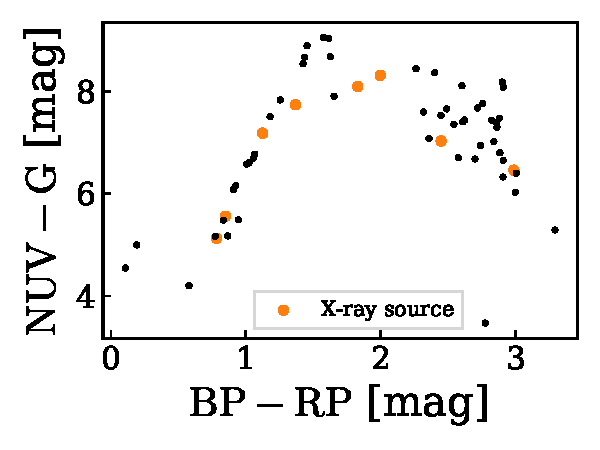
\includegraphics{nuv_xray.pdf}
  \caption{$\mathrm{NUV}-\mathrm{G}$ colors of 62 \galex\ cross-matched
    candidate members in \groupTen\ as a function of their \bprp\ color.
    }
  \label{fig:nuv}
\end{figure}

Young low-mass stars with a substantial convective layer stand out from
field stars in their enhanced UV and X-ray emission
as a result of strong internal magnetic dynamo coupled with rapid rotation
enhancing chromospheric and coronal activity
\citep{2004ARA&A..42..685Z,2008hsf2.book..757T,2011ApJ...727....6S,2013ApJ...774..101R}.
Thus, the UV and X-ray photometry can provide an independent indication of youth
for young stars in a coeval moving group.
We checked the UV and X-ray detection of
the candidate members by cross-mathing to the \galex\ source catalog
\citep{2005ApJ...619L...1M} and the \rosat\ all-sky survey
\citep[2RXS;][]{2016A&A...588A.103B}.
We used $2\arcsec$ and $20\arcsec$ search radius for \galex\ and 2RXS respectively.
When there are multiple \galex\ matches to a source, we choose the one with
the smallest NUV magnitude error.
We find that 62 of our candidate members ($\sim30$\%) have corresponding \galex\
UV detection, of which 10 are also X-ray sources.
There are 4 additional X-ray detected candidate members without UV detection.
The $\mathrm{NUV}-\mathrm{G}$ colors of the candidate members tend
to be at the edge of the distribution of field stars\footnote{
  White dwarfs, which extends to even bluer colors (lower left), have been removed
  from the field sample for \figname~\ref{fig:nuv} with a simple cut in
  \bprp\ vs. $M_G$ color-magnitude diagram ($M_G< 3(\bprp+0.5)+7.5$ if $\bprp<2$).
}
at fixed \bprp\ colors towards brighter
$\mathrm{NUV}$ magnitudes or show UV excess (\figname~\ref{fig:nuv}).
This is commonly seen in young stars upto ages of a few Myr old,
providing an indepdenent qualitative confirmation of the the isochrone age.

\subsection{Mean velocity and velocity dispersion}
\label{sec:fitting}

In this section, we derive the mean velocity and velocity dispersion of the
group using either only parallaxes and proper motions or full 6D information
including radial velocities.
Although the original selection was done by selecting comoving pairs, we can
also model the proper motions of the stars in the group as drawn from a single
mean velocity and a dispersion.
Historically, the basic assumption of a group of stars having the same velocity
has been used to derive a distance to the group (moving cluster method).
% or define the membership of each star.
However, given the exquisite measurements of parallaxes and proper motions via
astrometry, a forward modeling of the same basic model may yield interesting
inferences of geometric radial velocities of the group or other residual
velocity patterns beyond the simple isotropic dispersion
\citep{1999A&A...348.1040D,2002A&A...381..446M}

Here, we fit the simplest model of single isotropic Gaussian component to the data.
The components of the model are:
\begin{itemize}
  \item We assume that the velocity $\vec{v}_i$ of the star $i$ is drawn from
    a single Gaussian component with mean (group) velocity $\vec{u}$ and
    an isotropic dispersion $\sigma_{u}$:
    $$\vec{v}_i \sim \normal(\vec{u},\,\sigma_{u}).$$
    Then, the proper motion of star $i$ is
    $\transp{(\pmra,\,\pmdec)} = \mat{M}_i(\alpha_i,\,\delta_i) \vec{v}_i / r_i$ where
    $\mat{M}_i$ is the rotation matrix that transforms the equatorial
    rectangular coordinates to the tangential coordinates at the location
    $(\mathrm{R.A.},\,\mathrm{Decl.}) = (\alpha_i,\,\delta_i)$.

  \item We assume that the noise model for the \gaia\ data is Gaussian, and
    the covariance matrix $\mat{C_i}$ is given and fixed:
    $$(\tilde\varpi_i,\,\tilde\mu_{\alpha,i}^*,\,\tilde\mu_{\delta,i}) \sim
      \normal((\varpi_i,\,\mu_{\alpha,i}^*,\,\mu_{\delta,i}),\,\mat{C_i})$$

  \item \emph{Priors}:
    We assume an uninformative uniform prior in distance and a broad Gaussian
    prior $\vec{u} \sim \normal(0,\,100~\kms)$ and $\sigma_u \sim \normal(0, 50~\kms)$
    for the mean velocity $\vec{u}$ and velocity dispersion $\sigma_u$.
    Given that the parallax signal-to-noise is very high (median of 170),
    the distance prior has little effect on the fit.
\end{itemize}

This can be naturally extended to include radial velocities of each star.
In this case, the radial velocity is just $v_{r,i} =
\hat{\vec{u}}_r(\alpha_i,\,\delta_i) \cdot \vec{v}_i$
where $\hat{\vec{u}}_r(\alpha_i,\,\delta_i)$ is the unit radial vector
and the covariance of the noise model
is extended as $\mathrm{diag}(\mat{C_i},\,\sigma_{v_r}^2)$.
We refer the model using proper-motions only of all candidate member stars as `PM only'
and the model using a subset of 38 stars with RVs as `PM+RV' respectively.
For each case, we first do an optimization using L-BFGS algorithm starting from
the initial values $d_{i,0} = 1/{\tilde \varpi_i}$, a random mean velocity
$\vec{u}_0$ and $\sigma_u=10$~\kms.
We then sample the posterior distribution of $d_i$, $\vec{u}$ and $\sigma_u$
starting from this optimum.

This fitting achieves two main goals.
First, it properly deconvolves the uncertainty of each measurements taking
covariances between parallax and proper motions into account.
Secondly, for `PM only' case, this derives the geometric (astrometric) velocity
of the group, which can be compared to the spectroscopic RVs from \gaia\ DR 2
for a subset of stars.
This may be particularly interesting as \groupTen\ has a large angular span
($(\Delta\mathrm{R.A.},\,\Delta\mathrm{Decl.})\approx(39,\,18)$~deg)
and the astrometric precision is generally excellent.


\begin{figure}
  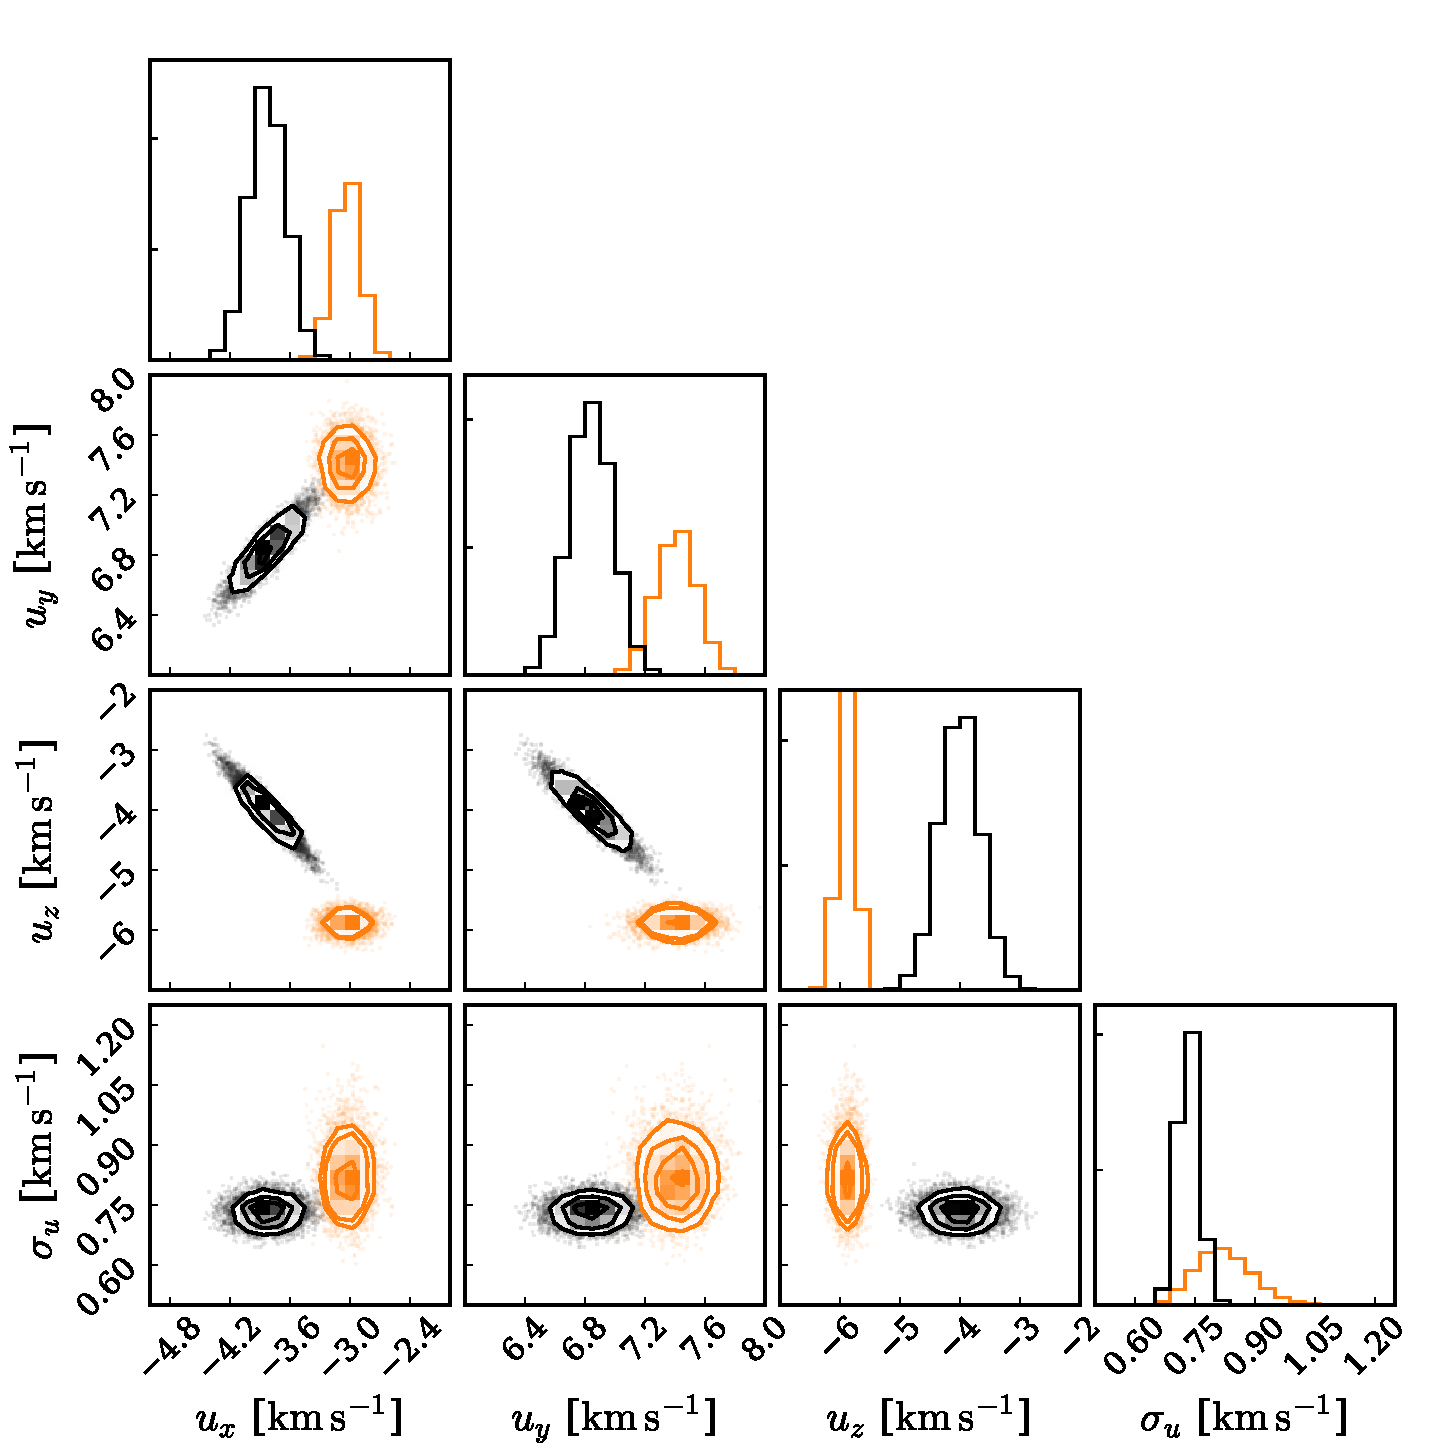
\includegraphics[width=0.95\linewidth]{isotropic.pdf}
  \caption{Fitting mean velocity and isotropic velocity dispersion of \groupTen\
    using astrometric parameters only (black) and including RVs for a subset
    of stars (orange).
    Geometric contraints on all three components of the velocities are in good
    agreement with those determined by including spectroscopic RVs.
    The velocities are in equatorial coordinates.
    }
  \label{fig:fit}
\end{figure}

\figname~\ref{fig:fit} summarizes and compares the fit result for the two cases.
Because this group spans a large area on sky, all three components of the mean
velocity is well-contrained geometrically using proper-motions only
(black density and contours).
The mean and standard deviation of the posterior samples of the mean velocity $\vec{u}$
is $(u_x,\,u_y,\,u_z) = (-3.82\pm0.19,\,6.84\pm0.14,\,-4.00\pm0.34)$ in
equatorial coordinates.
The velocity dispersion is very small with the mean of the posterior samples at
$\approx 0.73$~\kms.
The fit result of `PM only' is in good agreement with `PM+RV' case
with the mean velocity of $(-3.02\pm0.13,\,7.41\pm0.14,\,-5.89\pm0.13)$ and
the mean dispersion of $0.82$~\kms (orange density and contours).
While the differences between the two models is significant formally,
the difference is very small $<1$~\kms.

\subsection{Morphology}

\begin{figure}
  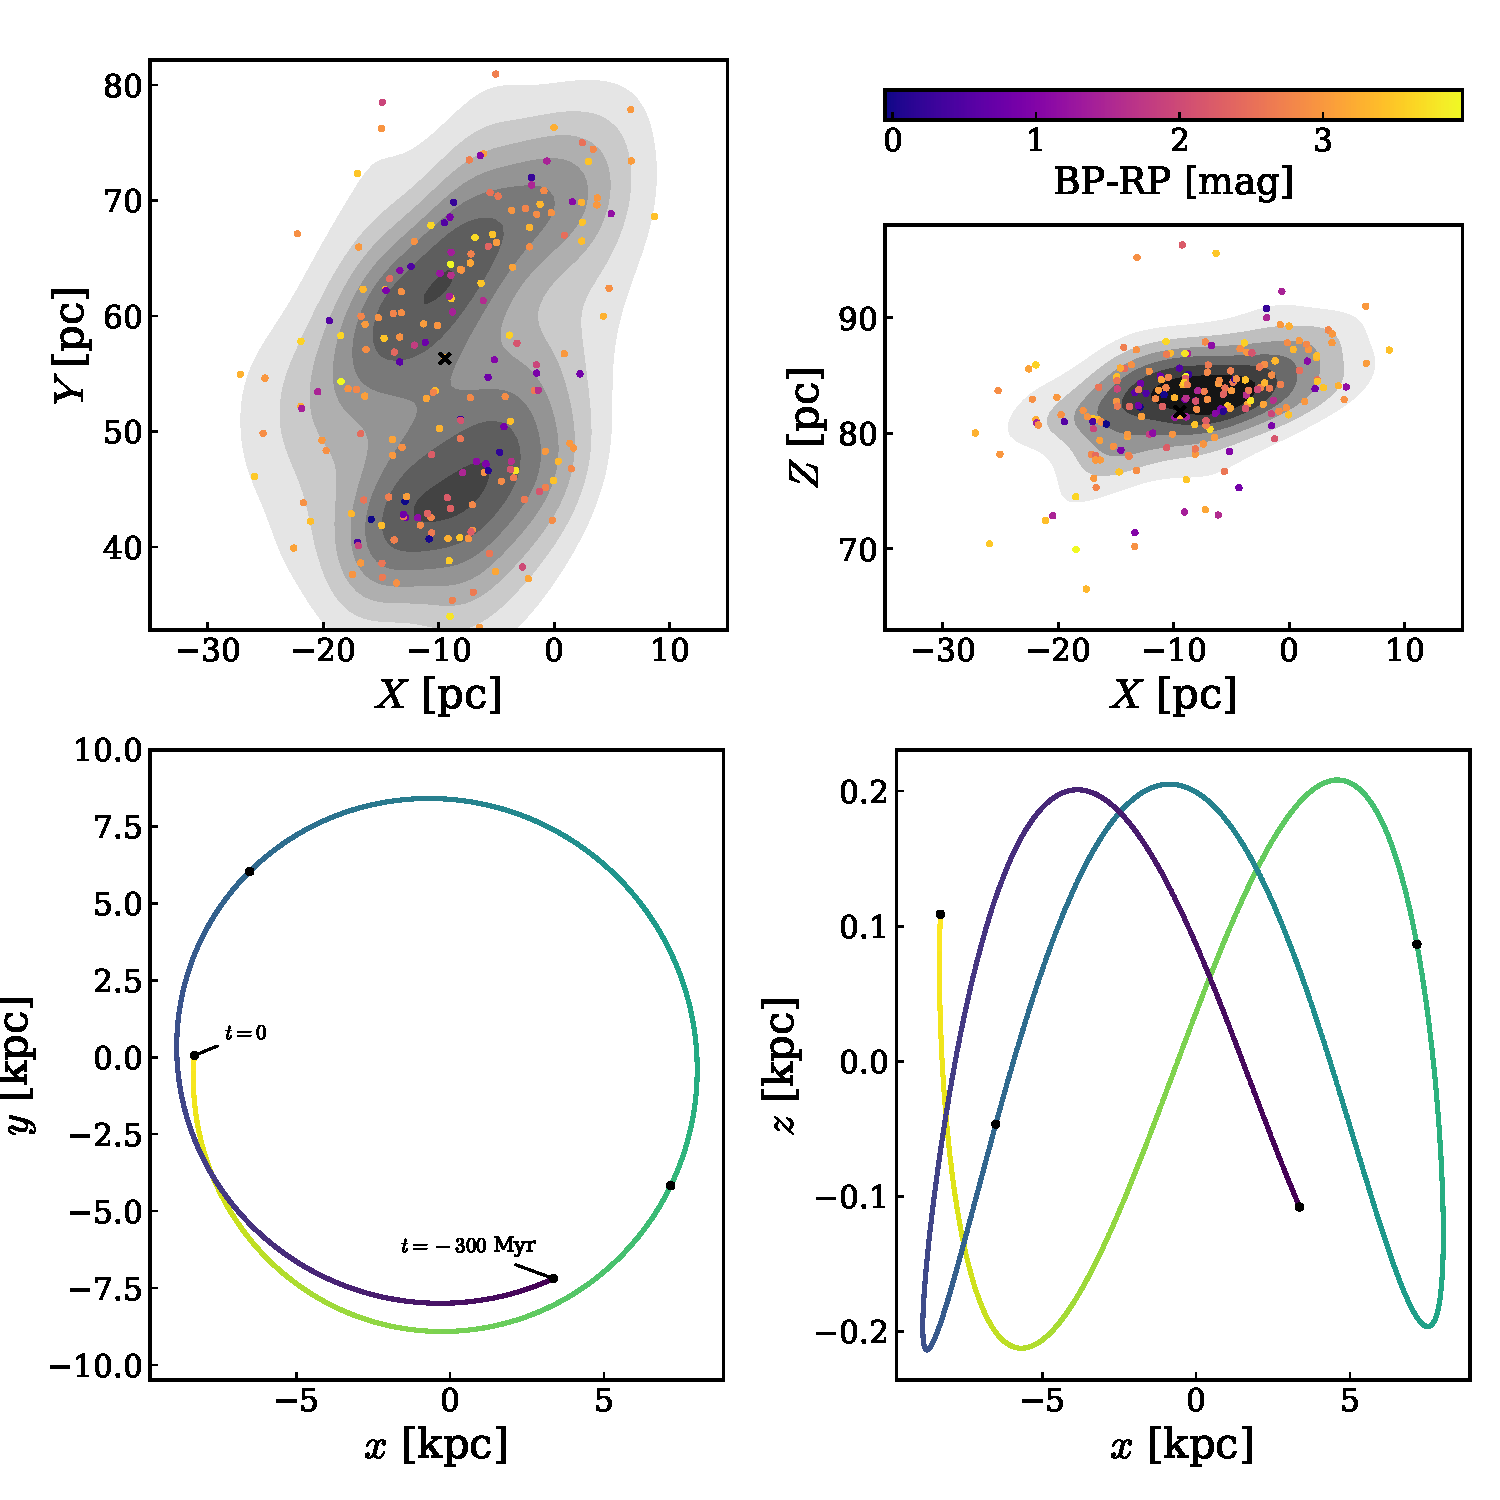
\includegraphics[width=0.95\linewidth]{orbit_morphology.pdf}
  \caption{Distribution of candidate members in \groupTen\ in
    the Galactic coordinates (top row) and the orbit of the group
    integrated backwards in
    a fiducial Milky Way potential (bottom row).
    On top row, stars are colored by their \bprp\ color, and
    the mean velocity is marked by an arrow in each projection.}
  \label{fig:orbit_morphology}
\end{figure}

The distribution of candidate members show no discernable center or
contentration in the Galactic $X$-$Y$ coordinates while it seems highly
concentrated in $Z$ direction around the median height of $\approx 82$~pc above
the Galactic plane (Figure~\ref{fig:orbit_morphology}).
The nominal standard deviation in $X$, $Y$, and $Z$ coordinates
is $6.7$, $10$, and $4.3$ pc respectively.
Furthermore, the candidate members seem to be divided in their $X$-$Y$
distribution, leaving a band of gap that is tilted with respect to the direction
of Galactic rotation ($+Y$).
The bottom panels of \figname~\ref{fig:orbit_morphology} shows the
nearly-circular orbit of the group integrated backwards for $300$~Myr in a Milky
Way potential \citep{2015ApJS..216...29B} using the mean velocity derived from
`PM+RV' model fitting in \sectionname~\ref{sec:fitting} and the median position
marked by a black `x' in the top panels of the same \figname.

We can roughly estimate the total mass of the group using BP-RP colors
and a model isochrone assuming an initial mass function (IMF).
We interpolate the BP-RP color-initial mass relation of a PARSEC isochrone of
solar metallicity and $\log\mathrm{age}=8.4$.
We select stars in a color range $0<\mathrm{BP-RP}<3$ which corresponds to
initial masses of $2.1~M_\odot$ and $0.24~M_\odot$.
For the Kroupa initial mass function \citep{2001MNRAS.322..231K},
the total mass is 2.4 times the mass within this color (mass) range.
Since the total mass of 124 candidate members within this color range is
$70~M_\odot$, the total mass is estimated to be $\approx167~M_\odot$.
This is likely a lower limit because
the membership selection may not be complete while the contamination is expected
to be low and because binarities are not taken into account.

% The group is unlikely to be graviationally bound.
% From kernel density estimation of the
% the $XYZ$ coordinates of the candidate members,
% the number density of the group in the densest region is $\approx0.03~\pc^{-3}$.

We speculate on the origin of the morphology of the group,
which is reminiscent of tidal tails.
One trivial possibility is that this particular group simply formed this way and
has not had the time to disperse yet.
Unlike the classical open clusters, for the smaller local associations of young stars
with typical ages less than 100 Myr,
it is often assumed that the gravitational interaction between member stars
is not important, and their dynamics is governed by the initial condition and
the Galactic potential \citep{1997MNRAS.285..479B,2018arXiv180300573M}.
Based on these assumptions, tracing back the orbits of the stars to a converging point
can result in a dynamical estimate of their ages.
However, simple expansion does not offer any explanation for the presense of the game
nor the highly anisotropic stretch of the morphology of \groupTen.
The age of \groupTen\ is significantly older than most local associations to
which such analysis is applied, which typically are tens of Myr old.
Given the velocity dispersion of $0.6$~\kms\ and an age of $200$~Myr,
if the group has been expanding shortly after the star formation,
it should now be spread over $>120$~pc.
While it is possible that there are more potential members of the group
beyond the search region defined here, the majority of the group is contained within
the extent of \figname~\ref{fig:orbit_morphology}.

Star clusters that survive the infant mortality are thought to be eventually
disrupted by the Galactic tidal field or encounters with Giant Molecular Clouds
(GMCs).
As stars in a cluster gain energy from external perturbations, they escape
primarily through $L_1$ and $L_2$ Lagrange points (Heggie 2001), which are
separated by $2r_J$ where $r_J$ is the tidal (or Jacobi) radius of the cluster.
For a cluster like \groupTen\ in the Solar neighborhoood with nearly circular orbit,
the tidal radius due to the Galactic tides is \citep{2010ARA&A..48..431P}
\begin{equation}
  \begin{split}
    r_J &= \left(\frac{G M}{2 (V_G/R_G)^2}\right)^{1/3}\\
        &= 8.5~\mathrm{pc} \left(\frac{M}{200~M_\odot}\right)^{1/3}
          \left(\frac{8.3~\mathrm{kpc}}{R}\right)^{2/3}
          \left(\frac{V}{220~\kms}\right)^{2/3}
  \end{split}
\end{equation}
Thus, the size of the gap between two streams of stars is roughly consistent with
$2r_J$.
The stars that leave the cluster potential through the two Lagrange points, which
are always aligned with the Galactic center, will then move away with velocities
close to the mean velocity of the cluster.
However, as indicated by the arrows in \figname~\ref{fig:orbit_morphology}, the
stretch of the group in $X-Y$ coordinates is significantly tilted from the mean
velocity although it does agree in $X-Z$ coordinates.
Furthermore, it is unclear whether a small cluster under the influence of the
Galactic tides throughout its lifetime of $\gtrsim 200$~Myr should still be
detectable as an overdensity in velocity space.
Whether the disruption was solely driven by the Galactic tides or was also
affected by passing GMCs, it is unclear why there is no clear progenitor
overdensity unless this is the final stage of disruption.
Further investigation is needed to illuminate the significance and origin of
this morphology.


% \subsection{Comparison to other groups}



\section{Summary}
\label{sec:discussion}

We confirmed and characterized a new nearby coeval comoving group first detected
in the Tycho-Gaia Astrometric Solution (\tgas) of \gaia\ DR 1 with
the independent and much improved data of \gaia\ DR 2.
We select a total of 194 candidate members with DR 2 astrometry
vastly improving the census of the group which was originally detected as
interconnected comoving pairs of 29 stars.
The age of the group is estimated to be $\approx200-250$~Myr from
matching the \gaia\ color-magnitude diagram with theoretical isochrones.
Some of the candidate members show independent sign of youth in their
UV and X-ray properties.
The group, which standed out from our previous search as the largest nearby
coeval moving group with little prior discussion in the literature,
shows an interesting morphology in their Galactic $X-Y$ distribution
which looks like broad tidal tails separated by an underdensity.
While we speculate on the possibility that the morphology may be related
to the disruption of a small star cluster,
not all features are easily explained and further
observational and theoretical investigation is needed.
This work is one step forward towards completing the census of
coeval moving groups in the Solar neighborhood.




\acknowledgements % simbad
This research has made use of the SIMBAD database,
operated at CDS, Strasbourg, France.
% ads
This research has made use of NASA's Astrophysics Data System.
% gaia
This work has made use of data from the European Space Agency (ESA) mission
{\it Gaia} (\url{https://www.cosmos.esa.int/gaia}), processed by the {\it Gaia}
Data Processing and Analysis Consortium (DPAC,
\url{https://www.cosmos.esa.int/web/gaia/dpac/consortium}). Funding for the DPAC
has been provided by national institutions, in particular the institutions
participating in the {\it Gaia} Multilateral Agreement.
% gaia sprints

% tremiane, francisca, erkal


\bibliography{refs}

\end{document}
